\chapter{Chemistry}
\section{A Chemical Background}
\begin{definition}
    Chemistry is the study of matter and the changes that material substances undergo.
\end{definition}

There are different uses in chemistry that coincide directly with mathematics. Within chemistry, there are different visual representations utilized to symbolize different chemical structures. For example, there exists a form of illustration called the ``Lewis Dot Structure.''
\begin{figure}[h]
         \centering
         
\includegraphics[width = 1.0in]{LS.png}
         \caption{\small{The Lewis Structure of a methane molecule.}}
  \end{figure}

The Lewis Structure of a molecule shows how the valence electrons are arranged among the atoms in the molecule. There exist rules which govern the formation of Lewis Structures for molecules.  The most important rule for the formation requires the molecule to achieve noble gas configuration. {\color{red}(cite)} An example of a Lewis Dot Structure can be seen in Figure 3.1. This means the molecule attains a total of eight valence electrons around the elements within the molecule. 
 \begin{figure}[h]
         \centering
         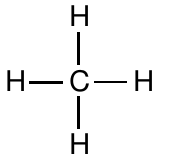
\includegraphics[width = 1.0in]{23.png}
         \caption{\small{The molecular structure of methane.}}
 \end{figure}
\par The two dots represent a bond between the elements and can be replaced with a line. Figure 3.2 demonstrates this concept. 
\par The illustration can translate to a mathematical graph that can be evaluated for the amount of walks that can be done throughout the structure. As mentioned before in the previous chapter, the graphs are used in combinatorics to count the number of closed walks.  Thus, we can apply our knowledge of combinatorics to molecular structures and see if a pattern presents itself. 

\section{Combinatorics and Chemistry}
Combinatorics can be used to explore chemical molecular structures.  Similar to the mathematical graphs seen throughout previous chapters, there is a relationship that molecular bonds share that can be used within combinatorics.  There are different types of structures that can represent a bond between elements.  
